% =====================================================================
%  THEORY GUIDE  --  Section 5 of the Extended Essay explained step by step
%  (study notes, not part of the essay)
%  Build:  tectonic -X compile theory_guide.tex   or  pdflatex x2
% =====================================================================
\documentclass[11pt,a4paper]{article}
\usepackage[a4paper,margin=2.3cm]{geometry}
\usepackage[T1]{fontenc}
\usepackage[utf8]{inputenc}
\usepackage{lmodern}
\usepackage{amsmath,amssymb,bm}
\usepackage{booktabs,array}
\usepackage{enumitem}
\usepackage{xcolor}
\usepackage{tikz}
\usetikzlibrary{decorations.pathmorphing,arrows.meta,calc,positioning,patterns,shapes.geometric}
\usepackage{pgfplots}
\pgfplotsset{compat=1.18}
\usepackage{tcolorbox}
\tcbuselibrary{skins,breakable}
\usepackage[hidelinks]{hyperref}

\newcommand{\muz}{\mu_0}
\newcommand{\mum}{\mu_{\mathrm m}}
\newcommand{\dd}{\mathrm{d}}
\newcommand{\un}[1]{\,\mathrm{#1}}
\newcommand{\Y}{Y}

\newtcolorbox{idea}{colback=blue!4,colframe=blue!55!black,title=Idea in one sentence,fonttitle=\bfseries,breakable}
\newtcolorbox{result}{colback=green!5,colframe=green!45!black,title=Result of this step,fonttitle=\bfseries,breakable}
\newtcolorbox{pitfall}{colback=red!4,colframe=red!60!black,title=Common confusion,fonttitle=\bfseries,breakable}
\newtcolorbox{ownwords}{colback=yellow!8,colframe=orange!80!black,title=What to say in your own words,fonttitle=\bfseries,breakable}
\newtcolorbox{selfcheck}{colback=gray!6,colframe=gray!60!black,title=Check yourself,fonttitle=\bfseries,breakable}

\title{\textbf{The theory of the coupled magnetic--mechanical oscillator}\\[4pt]
\large Section 5 of the Extended Essay, explained step by step}
\author{Study notes to accompany the essay draft}
\date{}

\begin{document}
\maketitle

\noindent These notes go through the theoretical model of the essay (Section~5) one logical step at a time, with a diagram for every step. Each step has the same layout: the \emph{idea} in one sentence, the \emph{maths}, the \emph{result}, and a box saying what you need to convey when you write it in your own words. The maths is exactly the same as in the essay; only the explanations are longer. Read the flow chart first: every later section is one box of it.

\section*{The whole argument on one page}

\begin{center}
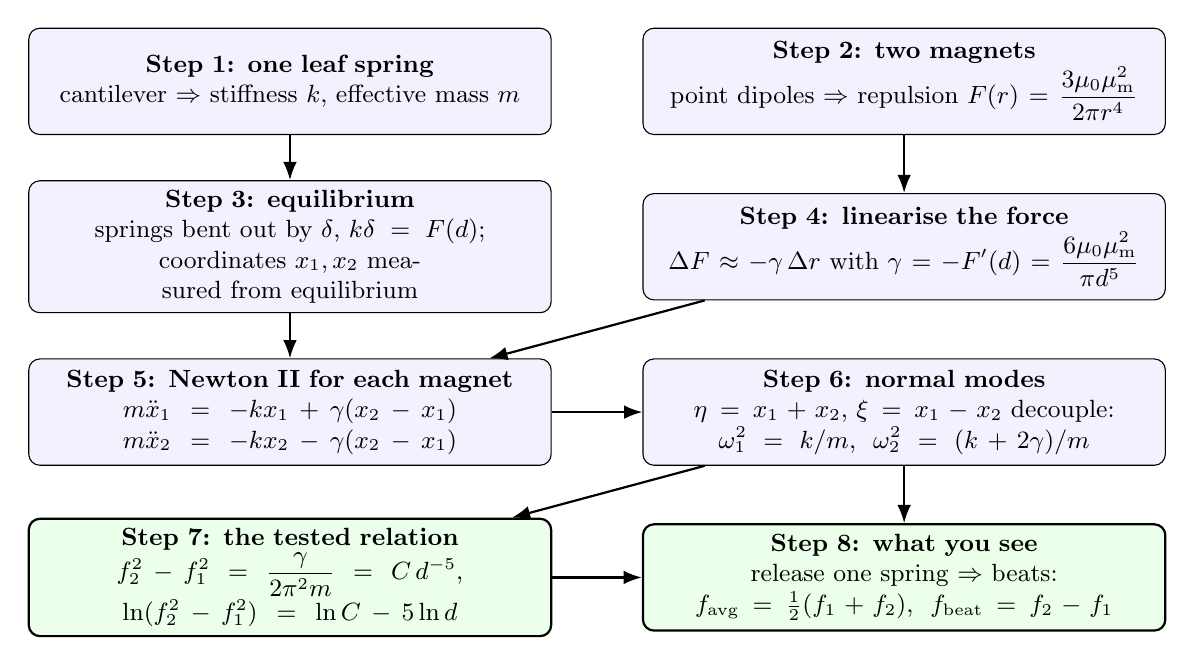
\begin{tikzpicture}[
  box/.style={draw,rounded corners,align=center,fill=blue!5,text width=6.4cm,minimum height=1.35cm,font=\small},
  res/.style={box,fill=green!8,thick},
  arr/.style={-{Latex},thick}]
\node[box] (A) at (0,0)     {\textbf{Step 1: one leaf spring}\\ cantilever $\Rightarrow$ stiffness $k$, effective mass $m$};
\node[box] (B) at (7.8,0)   {\textbf{Step 2: two magnets}\\ point dipoles $\Rightarrow$ repulsion $F(r)=\dfrac{3\muz\mum^2}{2\pi r^4}$};
\node[box] (C) at (0,-2.1)  {\textbf{Step 3: equilibrium}\\ springs bent out by $\delta$, $k\delta=F(d)$;\\ coordinates $x_1,x_2$ measured from equilibrium};
\node[box] (D) at (7.8,-2.1){\textbf{Step 4: linearise the force}\\ $\Delta F\approx-\gamma\,\Delta r$ with $\gamma=-F'(d)=\dfrac{6\muz\mum^2}{\pi d^5}$};
\node[box] (E) at (0,-4.2)  {\textbf{Step 5: Newton II for each magnet}\\ $m\ddot x_1=-kx_1+\gamma(x_2-x_1)$\\ $m\ddot x_2=-kx_2-\gamma(x_2-x_1)$};
\node[box] (F) at (7.8,-4.2){\textbf{Step 6: normal modes}\\ $\eta=x_1+x_2$, $\xi=x_1-x_2$ decouple:\\ $\omega_1^2=k/m$, $\ \omega_2^2=(k+2\gamma)/m$};
\node[res] (G) at (0,-6.3)  {\textbf{Step 7: the tested relation}\\ $f_2^2-f_1^2=\dfrac{\gamma}{2\pi^2m}=C\,d^{-5}$, $\ \ln(f_2^2-f_1^2)=\ln C-5\ln d$};
\node[res] (H) at (7.8,-6.3){\textbf{Step 8: what you see}\\ release one spring $\Rightarrow$ beats:\\ $f_{\rm avg}=\tfrac12(f_1+f_2)$, $\ f_{\rm beat}=f_2-f_1$};
\draw[arr] (A) -- (C);
\draw[arr] (B) -- (D);
\draw[arr] (C) -- (E);
\draw[arr] (D) -- (E);
\draw[arr] (E) -- (F);
\draw[arr] (F) -- (G);
\draw[arr] (F) -- (H);
\draw[arr] (G) -- (H);
\end{tikzpicture}
\end{center}

\noindent The logic is: \emph{mechanics gives $k$ and $m$; magnetism gives $F(r)$; linearising $F$ turns the magnetic repulsion into a third spring of stiffness $\gamma$; two masses joined by three springs have two normal modes; the difference of the squared mode frequencies depends only on $\gamma/m$, and $\gamma\propto d^{-5}$.}

\clearpage
\section{Step 1: a leaf spring with a magnet is a mass on a spring}

\begin{idea}
A clamped strip pushed sideways at its free end pushes back with a force proportional to the deflection (Hooke's law), so the tip behaves like a spring of stiffness $k$; the magnet plus part of the strip is the mass $m$ on that spring.
\end{idea}

\subsection*{1a. The stiffness $k$}

\begin{center}
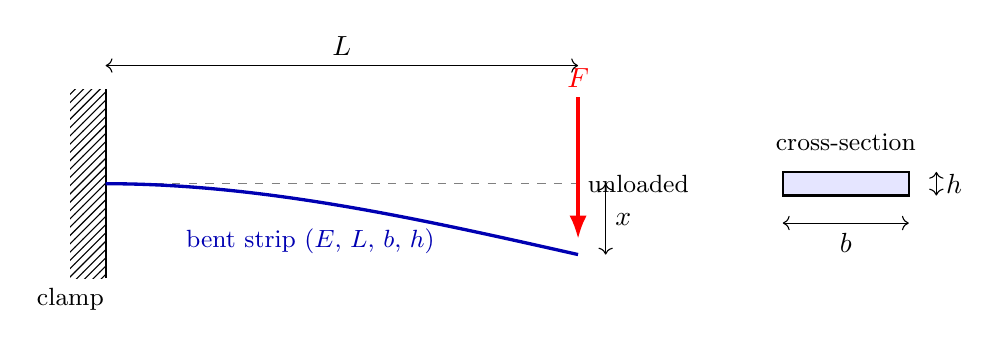
\begin{tikzpicture}[scale=1]
\fill[pattern=north east lines] (-0.45,-1.2) rectangle (0,1.2);
\draw[thick] (0,-1.2)--(0,1.2);
\node[below left] at (0.1,-1.2) {\small clamp};
\draw[dashed,gray] (0,0)--(6,0) node[right,black]{\small unloaded};
\draw[very thick,blue!70!black,domain=0:6,samples=60,variable=\s] plot ({\s},{-0.9*(\s*\s*(18-\s))/432});
\node[blue!70!black,below] at (2.6,-0.45) {\small bent strip ($E$, $L$, $b$, $h$)};
\draw[<->] (6.35,0)--(6.35,-0.9) node[midway,right]{$x$};
\draw[-{Latex},red,very thick] (6,1.1)--(6,-0.7);
\node[red,above] at (6,1.1) {$F$};
\draw[<->] (0,1.5)--(6,1.5) node[midway,above]{$L$};
\begin{scope}[shift={(8.6,0)}]
\draw[thick,fill=blue!10] (0,-0.15) rectangle (1.6,0.15);
\draw[<->] (0,-0.5)--(1.6,-0.5) node[midway,below]{$b$};
\draw[<->] (1.95,-0.15)--(1.95,0.15) node[midway,right]{$h$};
\node[above] at (0.8,0.3){\small cross-section};
\end{scope}
\end{tikzpicture}\\[2pt]
{\small\textbf{Figure 1.} A cantilever: a strip of length $L$, width $b$, thickness $h$, clamped at one end and pushed sideways at the other. The tip moves by $x$.}
\end{center}

Engineering beam theory (the standard cantilever formula, derived in Appendix~A of the essay) says that for a tip force $F$
\begin{equation}
x=\frac{FL^3}{3EI},\qquad I=\frac{bh^3}{12}.
\end{equation}
Here $E$ is Young's modulus of the material (how stiff copper is) and $I$ is the \emph{second moment of area} of the cross-section, a purely geometrical number that says how well the shape resists bending. Rearranging, force divided by deflection is a constant, i.e.\ a spring constant:
\begin{equation}
\boxed{k=\frac{F}{x}=\frac{3EI}{L^3}=\frac{Ebh^3}{4L^3}}
\end{equation}
Two sanity checks that show the formula is sensible: doubling the length makes the spring $2^3=8$ times \emph{softer} (a long strip is floppy), doubling the thickness makes it $8$ times \emph{stiffer}, and doubling the width only doubles $k$ (two strips side by side).

\subsection*{1b. The mass $m$}

If the strip had no mass, the oscillating mass would just be the magnet, $M$. But the strip does have mass, and it moves too. The problem is that it does not all move equally: the part next to the clamp barely moves, the tip moves as much as the magnet (Figure~2).

\begin{center}
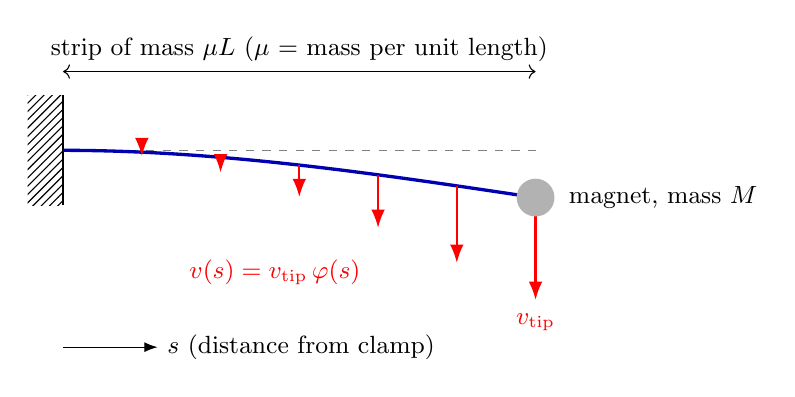
\begin{tikzpicture}[scale=1]
\fill[pattern=north east lines] (-0.45,-0.7) rectangle (0,0.7);
\draw[thick] (0,-0.7)--(0,0.7);
\draw[dashed,gray] (0,0)--(6,0);
\draw[very thick,blue!70!black,domain=0:6,samples=60,variable=\s] plot ({\s},{-0.6*(\s*\s*(18-\s))/432});
\foreach \s in {1,2,3,4,5,6}{
  \pgfmathsetmacro{\v}{1.3*(\s*\s*(18-\s))/432}
  \draw[-{Latex},red,thick] (\s,{-0.6*(\s*\s*(18-\s))/432}) -- ++(0,{-\v});
}
\node[red,below] at (6,-1.95) {\small $v_{\rm tip}$};
\node[red,anchor=east] at (3.9,-1.55) {\small $v(s)=v_{\rm tip}\,\varphi(s)$};
\fill[gray!60] (6,-0.6) circle (0.24);
\node[right] at (6.3,-0.6) {\small magnet, mass $M$};
\draw[<->] (0,1.0)--(6,1.0) node[midway,above]{\small strip of mass $\mu L$ ($\mu$ = mass per unit length)};
\draw[-{Latex}] (0,-2.5)--(1.2,-2.5) node[right]{\small $s$ (distance from clamp)};
\end{tikzpicture}\\[2pt]
{\small\textbf{Figure 2.} Rayleigh's idea. Every point of the strip moves with a velocity proportional to the static bending shape $\varphi(s)$ ($\varphi=0$ at the clamp, $\varphi=1$ at the tip). The strip's kinetic energy is the same as that of a point mass $\tfrac{33}{140}\mu L$ moving with the tip.}
\end{center}

\emph{Rayleigh's method} turns this into one number. Assume the strip vibrates in the same shape as its static deflection curve, $\varphi(s)=\dfrac{s^2(3L-s)}{2L^3}$, so that a point at distance $s$ from the clamp moves with velocity $v_{\rm tip}\varphi(s)$. Its kinetic energy is
\begin{equation}
K_{\rm strip}=\int_0^L\tfrac12\,\mu\,\big(v_{\rm tip}\varphi(s)\big)^2\,\dd s
=\tfrac12\Big(\mu\!\int_0^L\varphi^2\,\dd s\Big)v_{\rm tip}^2
=\tfrac12\Big(\tfrac{33}{140}\mu L\Big)v_{\rm tip}^2 .
\end{equation}
So, as far as kinetic energy is concerned, the strip behaves like a point mass $\tfrac{33}{140}\mu L\approx0.24\,\mu L$ sitting at the tip (the integral $\int_0^L\varphi^2\dd s=\tfrac{33}{140}L$ is just algebra with the cubic). The effective mass is therefore
\begin{equation}
\boxed{m=M+\tfrac{33}{140}\,\mu L}
\end{equation}
and a single spring on its own oscillates at $\omega_0=\sqrt{k/m}$, $f_0=\omega_0/2\pi$.

\begin{pitfall}
$m$ is \emph{not} the mass of the magnet, and \emph{not} the magnet plus the whole strip; it is the magnet plus about a quarter of the strip. If the magnet is much heavier than the strip the correction hardly matters, which is why heavy magnets make the lumped model accurate.
\end{pitfall}

\subsection*{1c. Why we measure $k$ and $m$ instead of calculating them}
The formulas contain $E$ (uncertain by $\sim10\%$ for rolled copper) and $h^3$ (a $3\%$ error in thickness becomes $9\%$ in $k$). So the formulas are used to \emph{understand} the system, while the numbers are \emph{measured}: plucking a spring with its own magnet (other magnet removed) gives $f_0=\frac1{2\pi}\sqrt{k/m}$ directly, and a load--deflection graph gives $k$; together they give $m$. For the exponent test (gradient $-5$) neither $k$ nor $m$ is needed at all, as Step~7 shows.

\begin{ownwords}
(1) A clamped leaf spring obeys Hooke's law at its tip, with $k=3EI/L^3$. (2) The oscillating mass is the magnet plus an effective fraction ($33/140$) of the strip, because the strip moves less near the clamp. (3) One spring alone is therefore a simple harmonic oscillator with $\omega_0^2=k/m$. (4) $k$ and $m$ are measured rather than calculated because $E$ and $h$ are poorly known.
\end{ownwords}

\bigskip
\section{Step 2: the force between the two magnets}

\begin{idea}
Seen from a few diameters away, a small magnet is a magnetic dipole; the field of a dipole falls as $1/r^3$, the force on a second dipole is proportional to the \emph{gradient} of that field, so the force between two facing magnets falls as $1/r^4$.
\end{idea}

\subsection*{2a. The field of one magnet on its axis}

\begin{center}
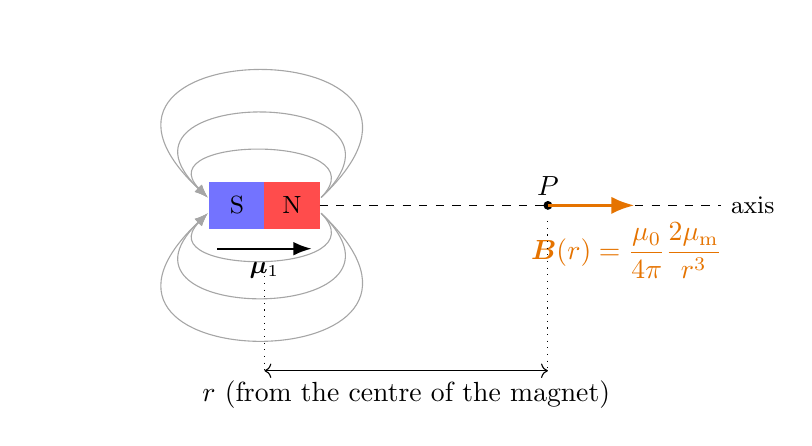
\begin{tikzpicture}[scale=1]
% field lines of a dipole pointing +x (drawn as ellipses through the poles)
\foreach \r in {1.0,1.7,2.5}{
  \draw[gray!70,-{Latex}] (0.72,0.1) .. controls (\r+0.5,\r*0.9) and (-\r-0.5,\r*0.9) .. (-0.72,0.1);
  \draw[gray!70,-{Latex}] (0.72,-0.1) .. controls (\r+0.5,-\r*0.9) and (-\r-0.5,-\r*0.9) .. (-0.72,-0.1);
}
\fill[blue!55] (-0.7,-0.3) rectangle (0,0.3);
\fill[red!70] (0,-0.3) rectangle (0.7,0.3);
\node at (-0.35,0){\small S}; \node at (0.35,0){\small N};
\draw[-{Latex},thick] (-0.6,-0.55)--(0.6,-0.55); \node[below] at (0,-0.6){\small $\bm\mu_1$};
\draw[dashed] (0.7,0)--(5.8,0) node[right]{\small axis};
\fill (3.6,0) circle (1.6pt); \node[above] at (3.6,0){$P$};
\draw[-{Latex},very thick,orange!90!black] (3.6,0)--(4.7,0);
\node[orange!90!black,below] at (4.6,-0.1){$\bm B(r)=\dfrac{\muz}{4\pi}\dfrac{2\mum}{r^3}$};
\draw[<->] (0,-2.1)--(3.6,-2.1) node[midway,below]{$r$ (from the centre of the magnet)};
\draw[dotted] (0,-0.9)--(0,-2.1); \draw[dotted] (3.6,-0.2)--(3.6,-2.1);
\end{tikzpicture}\\[2pt]
{\small\textbf{Figure 3.} A small magnet is a dipole of moment $\mum$. On its axis, at distance $r$ from its centre, the field points along the axis (away from the N pole outside the magnet) and has magnitude $\muz\,2\mum/(4\pi r^3)$.}
\end{center}

A permanent magnet is equivalent to a small current loop; its \emph{dipole moment} $\mum$ (units $\mathrm{A\,m^2}$) measures its strength. Along the axis of a loop of radius $a$ carrying current $I$, the Biot--Savart law gives $B=\muz Ia^2/\big(2(a^2+z^2)^{3/2}\big)$; far away ($z\gg a$) this becomes $B\approx\muz Ia^2/(2z^3)=\muz(I\pi a^2)/(2\pi z^3)$, and $I\pi a^2$ is the moment $\mum$. Hence
\begin{equation}
B(r)=\frac{\muz}{4\pi}\,\frac{2\mum}{r^3}\qquad\text{(on the axis, $r\gg$ size of the magnet).}
\end{equation}
The essential feature is the \emph{inverse cube}: the field of a dipole falls off one power faster than that of a single pole would. (For a real magnet, $\mum\approx B_{\rm r}V/\muz$ where $B_{\rm r}$ is the remanence quoted by the manufacturer and $V$ the volume; a $10\un{mm}\times3\un{mm}$ N42 disc has $\mum\approx0.24\un{A\,m^2}$.)

\subsection*{2b. The force on the second magnet}

\begin{center}
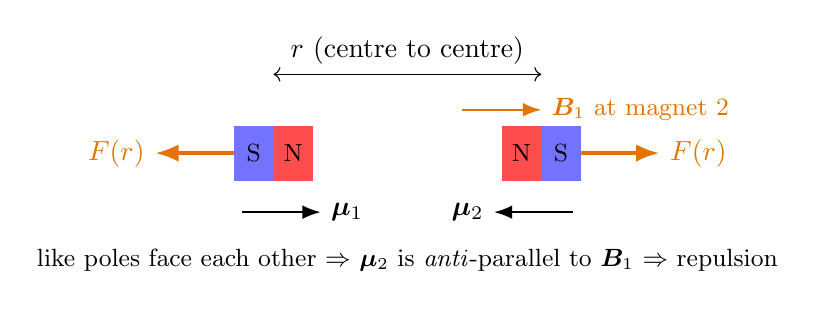
\begin{tikzpicture}[scale=1]
\fill[blue!55] (0,-0.35) rectangle (0.5,0.35); \fill[red!70] (0.5,-0.35) rectangle (1,0.35);
\node at (0.25,0){\small S}; \node at (0.75,0){\small N};
\fill[red!70] (3.4,-0.35) rectangle (3.9,0.35); \fill[blue!55] (3.9,-0.35) rectangle (4.4,0.35);
\node at (3.65,0){\small N}; \node at (4.15,0){\small S};
\draw[-{Latex},thick] (0.1,-0.75)--(1.1,-0.75) node[right]{$\bm\mu_1$};
\draw[-{Latex},thick] (4.3,-0.75)--(3.3,-0.75) node[left]{$\bm\mu_2$};
\draw[-{Latex},thick,orange!90!black] (2.9,0.55)--(3.9,0.55) node[right]{\small $\bm B_1$ at magnet 2};
\draw[<->] (0.5,1.0)--(3.9,1.0) node[midway,above]{$r$ (centre to centre)};
\draw[-{Latex},very thick,orange!90!black] (4.4,0)--(5.4,0) node[right]{$F(r)$};
\draw[-{Latex},very thick,orange!90!black] (0,0)--(-1,0) node[left]{$F(r)$};
\node[below] at (2.2,-1.1) {\small like poles face each other $\Rightarrow$ $\bm\mu_2$ is \emph{anti}-parallel to $\bm B_1$ $\Rightarrow$ repulsion};
\end{tikzpicture}\\[2pt]
{\small\textbf{Figure 4.} Two magnets on a common axis with like poles facing. The field of magnet 1 at magnet 2 points to the right; the moment of magnet 2 points to the left.}
\end{center}

A dipole $\bm\mu_2$ in a field $\bm B$ has potential energy $U=-\bm\mu_2\cdot\bm B$ (lowest when aligned with the field, like a compass needle). With like poles facing, $\bm\mu_2$ is anti-parallel to $\bm B_1$, so
\begin{equation}
U(r)=+\mum B_1(r)=\frac{\muz}{4\pi}\,\frac{2\mum^2}{r^3}.
\end{equation}
Force is minus the gradient of potential energy:
\begin{equation}
\boxed{F(r)=-\frac{\dd U}{\dd r}=\frac{\muz}{4\pi}\,\frac{6\mum^2}{r^4}=\frac{3\muz\mum^2}{2\pi\,r^4}}
\end{equation}
The sign is positive, meaning the force \emph{increases} $r$: repulsion. The physics behind the power: field $\propto r^{-3}$, force $\propto$ its derivative $\propto r^{-4}$.

\begin{pitfall}
The $r$ in $F(r)$ is the distance between the \emph{centres} of the two dipoles, not the gap between their faces. That is why the essay defines $d$ centre-to-centre ($d=\text{gap}+\text{thickness}$). And the dipole formula is only exact when $r$ is large compared with the magnet size $D$; at $r/D\approx2$ the real force falls \emph{less} steeply than $r^{-4}$ (essay Section~10.3).
\end{pitfall}

\begin{ownwords}
(1) Each magnet is modelled as a point dipole. (2) The on-axis field of a dipole is $\propto\mum/r^3$. (3) The energy of the second dipole in that field is $+\mum B$ because like poles face; differentiating gives a repulsive force $\propto\mum^2/r^4$. (4) The model needs $d\gg D$, which is only marginally true here.
\end{ownwords}

\bigskip
\section{Step 3: equilibrium and coordinates}

\begin{idea}
With both magnets mounted the repulsion bends each spring outwards by $\delta$ until $k\delta=F(d)$; all displacements are then measured from this bent equilibrium, and $d$ is the equilibrium centre-to-centre separation.
\end{idea}

\begin{center}
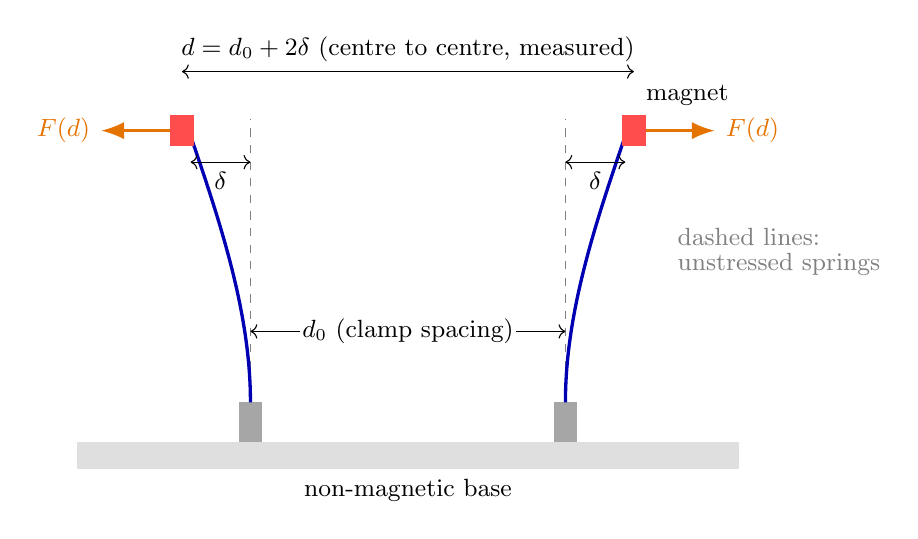
\begin{tikzpicture}[scale=1]
\fill[gray!25] (-4.2,-0.35) rectangle (4.2,0);
\node[below] at (0,-0.35) {\small non-magnetic base};
\foreach \sx in {-1,1}{
  \fill[gray!70] ({\sx*2.0-0.15},0) rectangle ({\sx*2.0+0.15},0.5);
  \draw[dashed,gray] ({\sx*2.0},0.5)--({\sx*2.0},4.1);
  \draw[very thick,blue!70!black,domain=0:3.5,samples=40,variable=\s]
        plot ({\sx*2.0+\sx*0.8*(\s*\s*(10.5-\s))/85.75},{0.5+\s});
}
\fill[red!70] (2.72,3.75) rectangle (3.02,4.15);
\fill[red!70] (-3.02,3.75) rectangle (-2.72,4.15);
\node[above right] at (2.9,4.15) {\small magnet};
\draw[<->] (-2.0,1.4)--(2.0,1.4) node[midway,fill=white,inner sep=1pt]{\small $d_0$ (clamp spacing)};
\node[gray,anchor=west] at (3.3,2.6) {\small dashed lines:};\node[gray,anchor=west] at (3.3,2.25) {\small unstressed springs};
\draw[<->] (-2.87,4.7)--(2.87,4.7) node[midway,above]{\small $d=d_0+2\delta$ (centre to centre, measured)};
\draw[<->] (2.0,3.55)--(2.76,3.55) node[midway,below]{\small $\delta$};
\draw[<->] (-2.76,3.55)--(-2.0,3.55) node[midway,below]{\small $\delta$};
\draw[-{Latex},orange!90!black,very thick] (3.02,3.95)--(3.9,3.95) node[right]{\small $F(d)$};
\draw[-{Latex},orange!90!black,very thick] (-3.02,3.95)--(-3.9,3.95) node[left]{\small $F(d)$};
\end{tikzpicture}\\[2pt]
{\small\textbf{Figure 5.} Equilibrium. The repulsion $F(d)$ pushes each tip outwards until the spring's restoring force $k\delta$ balances it.}
\end{center}

At rest each spring is bent outwards by $\delta$ with $k\delta=F(d)$. If the clamps are $d_0$ apart, the magnets sit at $d=d_0+2\delta$. Finding $d$ from $d_0$ would mean solving $k(d-d_0)/2=3\muz\mum^2/(2\pi d^4)$ for $d$---a fifth-degree equation with two unknown constants. The essay avoids this completely by \emph{measuring} $d$ directly at equilibrium (magnets mounted, springs already bent). From then on:
\begin{itemize}[nosep]
\item $x_1$, $x_2$ are the displacements of magnets 1 and 2 from their \emph{equilibrium} positions, both counted positive in the same direction (say to the right);
\item the instantaneous separation is $r=d+x_2-x_1$ (if magnet 2 moves right and magnet 1 does not, the gap grows).
\end{itemize}
Note the unstressed (straight) position of spring~1 is $\delta$ to the right of its equilibrium, and that of spring~2 is $\delta$ to the left; we will need this for the spring forces in Step~5.

\begin{ownwords}
Define $d$ as the equilibrium centre-to-centre separation, measured with both magnets in place; explain that this sidesteps the static bending $\delta$ (which would otherwise require solving a quintic) and that all displacements are measured from equilibrium.
\end{ownwords}

\section{Step 4: linearising the repulsion --- the magnetic ``spring'' $\gamma$}

\begin{idea}
For small movements the curved force law can be replaced by its tangent at $r=d$; the slope of that tangent is a stiffness, $\gamma=-F'(d)$: the magnetic repulsion behaves like a compressed spring between the magnets.
\end{idea}

\begin{center}
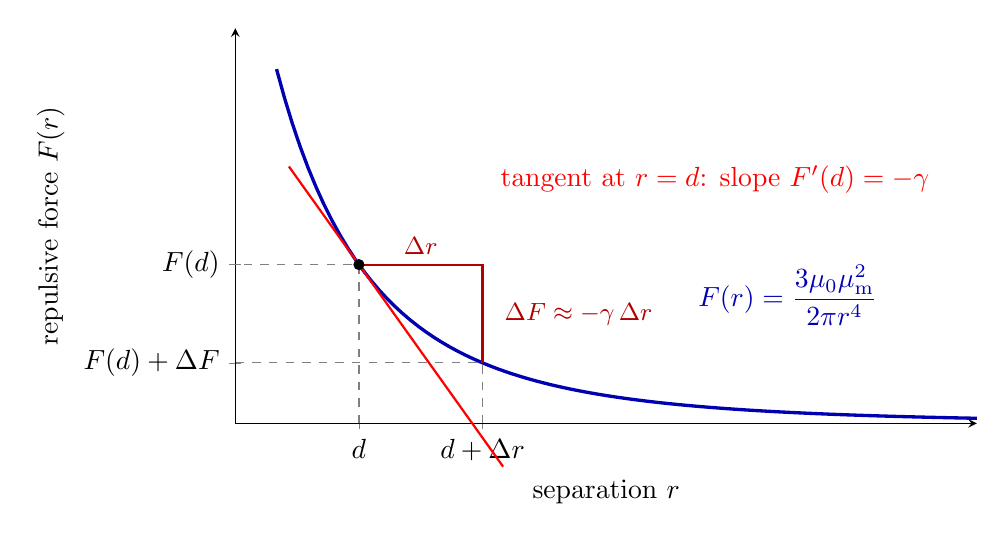
\begin{tikzpicture}
\begin{axis}[width=11cm,height=6.6cm,axis lines=left,
  xlabel={separation $r$},ylabel={repulsive force $F(r)$},
  xmin=0.8,xmax=2.6,ymin=0,ymax=1.7,
  xtick={1.1,1.4},xticklabels={$d$,$d+\Delta r$},ytick={0.683,0.26},yticklabels={$F(d)$,$F(d)+\Delta F$},
  clip=false]
\addplot[very thick,blue!70!black,domain=0.9:2.6,samples=90]{1/x^4};
\node[blue!70!black,anchor=west] at (axis cs:1.9,0.55){$F(r)=\dfrac{3\muz\mum^2}{2\pi r^4}$};
\addplot[red,thick,domain=0.93:1.45]{0.683-2.4837*(x-1.1)};
\node[red,anchor=west] at (axis cs:1.42,1.05){tangent at $r=d$: slope $F'(d)=-\gamma$};
\draw[dashed,gray] (axis cs:1.1,0)--(axis cs:1.1,0.683)--(axis cs:0.8,0.683);
\draw[dashed,gray] (axis cs:1.4,0)--(axis cs:1.4,0.26)--(axis cs:0.8,0.26);
\draw[red!70!black,thick] (axis cs:1.1,0.683)--(axis cs:1.4,0.683)--(axis cs:1.4,0.26);
\node[red!70!black,above] at (axis cs:1.25,0.683){\small $\Delta r$};
\node[red!70!black,anchor=west] at (axis cs:1.43,0.47){\small $\Delta F\approx-\gamma\,\Delta r$};
\addplot[only marks,mark=*,mark size=1.8pt,black] coordinates{(1.1,0.683)};
\end{axis}
\end{tikzpicture}\\[2pt]
{\small\textbf{Figure 6.} Linearisation. Near the equilibrium separation the force curve is replaced by its tangent. Moving the magnets $\Delta r$ further apart reduces the repulsion by $\gamma\Delta r$; pushing them closer increases it by the same amount---exactly what a compressed spring of stiffness $\gamma$ would do.}
\end{center}

Take the separation to be $r=d+u$ with $u$ small. A Taylor expansion to first order gives
\begin{equation}
F(d+u)\approx F(d)+F'(d)\,u,\qquad\text{so}\qquad F(d+u)-F(d)\approx-\gamma\,u,\quad \gamma\equiv-F'(d).
\end{equation}
Differentiating $F\propto r^{-4}$: $\dfrac{\dd}{\dd r}r^{-4}=-4r^{-5}$, hence
\begin{equation}
\boxed{\gamma=-\frac{\dd F}{\dd r}\bigg|_{r=d}=\frac{4F(d)}{d}=\frac{6\muz\mum^2}{\pi\,d^5}}
\end{equation}
$\gamma$ is called the \emph{magnetic stiffness}: the extra restoring force per unit change of separation. It is positive because a repulsion that \emph{weakens} with distance always pushes the magnets back towards their equilibrium separation---closer means a bigger push apart, further means a smaller push and the springs win. This is the single most important step in the whole theory: it is where the power $-5$ comes from (one more than the $-4$ of the force, because $\gamma$ is a derivative).

\begin{selfcheck}
What would change if the magnets \emph{attracted}? Then $F$ is negative and grows in magnitude as $r$ shrinks, so $\gamma=-F'(d)$ is \emph{negative}: the magnetic ``spring'' has negative stiffness and softens the anti-phase mode ($\omega_2<\omega_1$). If $2|\gamma|>k$ the equilibrium is unstable and the magnets snap together---which is exactly what happens with attracting magnets on floppy springs.
\end{selfcheck}

\begin{ownwords}
Explain that the displacements are small compared with $d$, so the force can be replaced by its tangent; that the slope of the tangent, $\gamma=-F'(d)=4F(d)/d$, is an effective spring constant; and that because $F\propto d^{-4}$, $\gamma\propto d^{-5}$.
\end{ownwords}

\bigskip
\section{Step 5: Newton's second law for each magnet}

\begin{idea}
Each magnet feels its own spring pulling it back and the magnetic force from the other magnet; writing $F=ma$ for both, with the linearised magnetic force, gives two coupled linear equations---the same equations as two masses joined by a spring of stiffness $\gamma$.
\end{idea}

\begin{center}
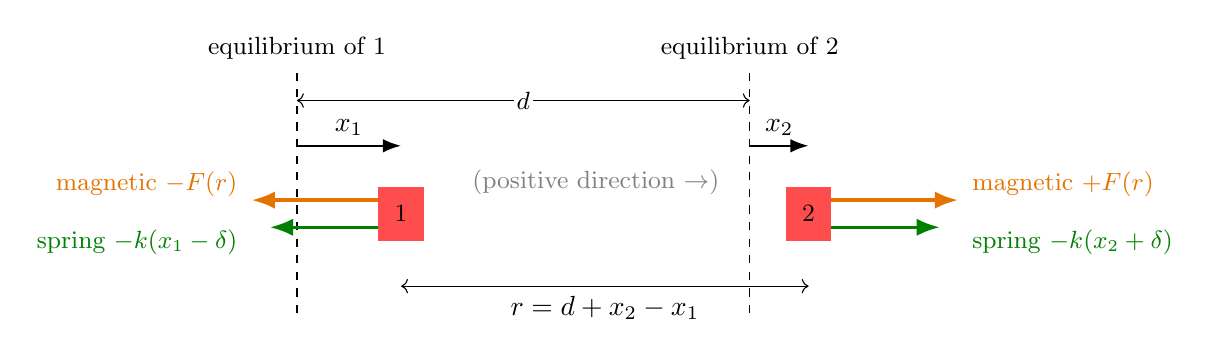
\begin{tikzpicture}[scale=1.15]
\draw[dashed] (0,-1.1)--(0,1.6); \node[above] at (0,1.6){\small equilibrium of 1};
\draw[dashed] (5,-1.1)--(5,1.6); \node[above] at (5,1.6){\small equilibrium of 2};
\fill[red!70] (0.9,-0.3) rectangle (1.4,0.3); \node at (1.15,0){\small 1};
\fill[red!70] (5.4,-0.3) rectangle (5.9,0.3); \node at (5.65,0){\small 2};
\draw[-{Latex},thick] (0,0.75)--(1.15,0.75) node[midway,above]{$x_1$};
\draw[-{Latex},thick] (5,0.75)--(5.65,0.75) node[midway,above]{$x_2$};
\draw[<->] (1.15,-0.8)--(5.65,-0.8) node[midway,below]{$r=d+x_2-x_1$};
\draw[<->] (0,1.25)--(5,1.25) node[midway,fill=white,inner sep=1pt]{\small $d$};
\draw[-{Latex},very thick,orange!90!black] (0.9,0.15)--(-0.5,0.15);
\node[orange!90!black,anchor=east] at (-0.55,0.32) {\small magnetic $-F(r)$};
\draw[-{Latex},very thick,green!50!black] (0.9,-0.15)--(-0.3,-0.15);
\node[green!50!black,anchor=east] at (-0.55,-0.32) {\small spring $-k(x_1-\delta)$};
\draw[-{Latex},very thick,orange!90!black] (5.9,0.15)--(7.3,0.15);
\node[orange!90!black,anchor=west] at (7.35,0.32) {\small magnetic $+F(r)$};
\draw[-{Latex},very thick,green!50!black] (5.9,-0.15)--(7.1,-0.15);
\node[green!50!black,anchor=west] at (7.35,-0.32) {\small spring $-k(x_2+\delta)$};
\node[gray] at (3.3,0.35) {\small (positive direction $\rightarrow$)};
\end{tikzpicture}\\[2pt]
{\small\textbf{Figure 7.} Free-body diagram (horizontal forces only). Both magnets shown displaced to the right. The spring force of each is proportional to the displacement from its \emph{unstressed} position, which is $+\delta$ for spring~1 and $-\delta$ for spring~2 (Figure~5). The magnetic force pushes magnet~1 to the left and magnet~2 to the right, with magnitude $F(r)$ evaluated at the \emph{current} separation.}
\end{center}

\textbf{Magnet 1.} Its displacement from the unstressed position is $x_1-\delta$, so the spring exerts $-k(x_1-\delta)$; the magnetic force is $-F(d+u)$ with $u=x_2-x_1$. Newton II:
\begin{align}
m\ddot x_1&=-k(x_1-\delta)-F(d+u)\notag\\
          &=-kx_1+\underbrace{k\delta}_{=F(d)}-F(d+u)
           =-kx_1+\big[F(d)-F(d+u)\big]\approx-kx_1+\gamma u .
\end{align}
The equilibrium condition $k\delta=F(d)$ has cancelled the constant part of the magnetic force; only the \emph{change} of the force, $-\gamma u$ from Step~4, survives. \textbf{Magnet 2} is the mirror image: spring force $-k(x_2+\delta)$, magnetic force $+F(d+u)$, giving $m\ddot x_2=-kx_2-\gamma u$. Together:
\begin{equation}
\boxed{\;m\ddot x_1=-kx_1+\gamma(x_2-x_1),\qquad m\ddot x_2=-kx_2-\gamma(x_2-x_1)\;}
\label{eq:eom}
\end{equation}

\begin{center}
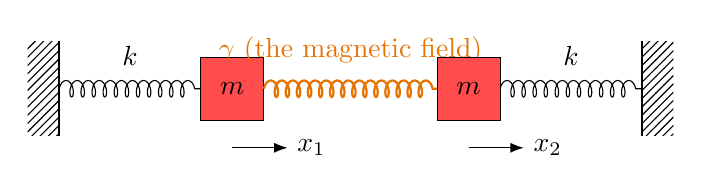
\begin{tikzpicture}[scale=1]
\fill[pattern=north east lines] (-0.4,-0.6) rectangle (0,0.6); \draw[thick](0,-0.6)--(0,0.6);
\draw[decorate,decoration={coil,aspect=0.5,segment length=4pt,amplitude=3pt}] (0,0)--(1.8,0) node[midway,above=5pt]{$k$};
\draw[fill=red!70] (1.8,-0.4) rectangle (2.6,0.4); \node at (2.2,0){$m$};
\draw[decorate,decoration={coil,aspect=0.5,segment length=4pt,amplitude=3pt},orange!90!black,thick] (2.6,0)--(4.8,0) node[midway,above=5pt]{$\gamma$ (the magnetic field)};
\draw[fill=red!70] (4.8,-0.4) rectangle (5.6,0.4); \node at (5.2,0){$m$};
\draw[decorate,decoration={coil,aspect=0.5,segment length=4pt,amplitude=3pt}] (5.6,0)--(7.4,0) node[midway,above=5pt]{$k$};
\fill[pattern=north east lines] (7.4,-0.6) rectangle (7.8,0.6); \draw[thick](7.4,-0.6)--(7.4,0.6);
\draw[-{Latex}] (2.2,-0.75)--(2.9,-0.75) node[right]{$x_1$};
\draw[-{Latex}] (5.2,-0.75)--(5.9,-0.75) node[right]{$x_2$};
\end{tikzpicture}\\[2pt]
{\small\textbf{Figure 8.} Mechanical equivalent of equations~\eqref{eq:eom}: two equal masses on equal springs $k$, joined by a third spring of stiffness $\gamma$. The middle spring exerts $\gamma(x_2-x_1)$ on the left mass and the opposite on the right mass---exactly the coupling terms.}
\end{center}

\begin{pitfall}
Students often write the magnetic force as $-\gamma x_1$. It is not: the magnetic force depends on the \emph{separation} $x_2-x_1$, not on where magnet~1 is. If both magnets move together ($x_1=x_2$) the separation does not change and the magnetic force does not change at all.
\end{pitfall}

\begin{ownwords}
Draw the free-body diagram, state the two forces on each magnet, apply Newton~II, use $k\delta=F(d)$ to remove the constant force, and use Step~4 to linearise. Point out that the result is identical to two masses coupled by a spring of stiffness $\gamma$.
\end{ownwords}

\bigskip
\section{Step 6: normal modes}

\begin{idea}
The two equations are decoupled by adding and subtracting them: the sum $x_1+x_2$ and the difference $x_1-x_2$ each obey a simple harmonic equation with its own frequency. These are the two normal modes.
\end{idea}

Add the two equations of \eqref{eq:eom}: the coupling terms cancel,
\begin{equation}
m(\ddot x_1+\ddot x_2)=-k(x_1+x_2)\quad\Longrightarrow\quad m\ddot\eta=-k\eta,\qquad \eta\equiv x_1+x_2 .
\end{equation}
Subtract them: the coupling terms add,
\begin{equation}
m(\ddot x_1-\ddot x_2)=-k(x_1-x_2)+2\gamma(x_2-x_1)=-(k+2\gamma)(x_1-x_2)
\ \Longrightarrow\ m\ddot\xi=-(k+2\gamma)\xi,\quad \xi\equiv x_1-x_2 .
\end{equation}
Each of $\eta$ and $\xi$ is a simple harmonic oscillator ($\ddot q=-\omega^2q$), so
\begin{equation}
\boxed{\;\omega_1^2=\frac{k}{m}\ \ (\text{in-phase},\ \eta),\qquad \omega_2^2=\frac{k+2\gamma}{m}\ \ (\text{anti-phase},\ \xi)\;}
\label{eq:modes}
\end{equation}

\begin{center}
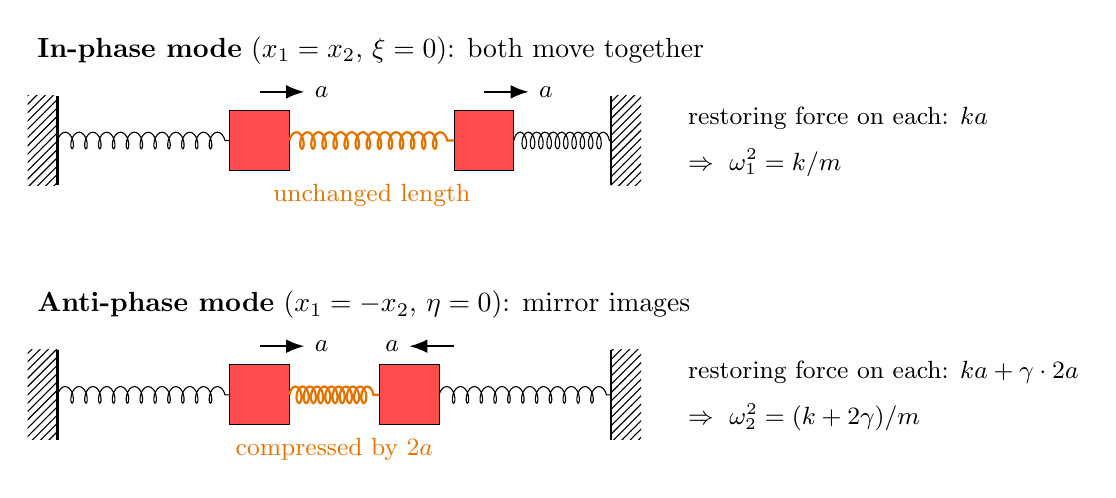
\begin{tikzpicture}[scale=0.95]
\begin{scope}
\node[anchor=west] at (-0.4,1.2){\textbf{In-phase mode} ($x_1=x_2$, $\xi=0$): both move together};
\fill[pattern=north east lines] (-0.4,-0.6) rectangle (0,0.6); \draw[thick](0,-0.6)--(0,0.6);
\draw[decorate,decoration={coil,aspect=0.5,segment length=5pt,amplitude=3pt}] (0,0)--(2.3,0);
\draw[fill=red!70] (2.3,-0.4) rectangle (3.1,0.4);
\draw[decorate,decoration={coil,aspect=0.5,segment length=4pt,amplitude=3pt},orange!90!black,thick] (3.1,0)--(5.3,0);
\node[orange!90!black,below] at (4.2,-0.45){\small unchanged length};
\draw[fill=red!70] (5.3,-0.4) rectangle (6.1,0.4);
\draw[decorate,decoration={coil,aspect=0.5,segment length=3pt,amplitude=3pt}] (6.1,0)--(7.4,0);
\fill[pattern=north east lines] (7.4,-0.6) rectangle (7.8,0.6); \draw[thick](7.4,-0.6)--(7.4,0.6);
\draw[-{Latex},thick] (2.7,0.65)--(3.3,0.65) node[right]{\small $a$};
\draw[-{Latex},thick] (5.7,0.65)--(6.3,0.65) node[right]{\small $a$};
\node[anchor=west] at (8.3,0.3){\small restoring force on each: $ka$};
\node[anchor=west] at (8.3,-0.3){\small $\Rightarrow\ \omega_1^2=k/m$};
\end{scope}
\begin{scope}[yshift=-3.4cm]
\node[anchor=west] at (-0.4,1.2){\textbf{Anti-phase mode} ($x_1=-x_2$, $\eta=0$): mirror images};
\fill[pattern=north east lines] (-0.4,-0.6) rectangle (0,0.6); \draw[thick](0,-0.6)--(0,0.6);
\draw[decorate,decoration={coil,aspect=0.5,segment length=5pt,amplitude=3pt}] (0,0)--(2.3,0);
\draw[fill=red!70] (2.3,-0.4) rectangle (3.1,0.4);
\draw[decorate,decoration={coil,aspect=0.5,segment length=2.6pt,amplitude=3pt},orange!90!black,thick] (3.1,0)--(4.3,0);
\node[orange!90!black,below] at (3.7,-0.45){\small compressed by $2a$};
\draw[fill=red!70] (4.3,-0.4) rectangle (5.1,0.4);
\draw[decorate,decoration={coil,aspect=0.5,segment length=5pt,amplitude=3pt}] (5.1,0)--(7.4,0);
\fill[pattern=north east lines] (7.4,-0.6) rectangle (7.8,0.6); \draw[thick](7.4,-0.6)--(7.4,0.6);
\draw[-{Latex},thick] (2.7,0.65)--(3.3,0.65) node[right]{\small $a$};
\draw[-{Latex},thick] (5.3,0.65)--(4.7,0.65) node[left]{\small $a$};
\node[anchor=west] at (8.3,0.3){\small restoring force on each: $ka+\gamma\cdot2a$};
\node[anchor=west] at (8.3,-0.3){\small $\Rightarrow\ \omega_2^2=(k+2\gamma)/m$};
\end{scope}
\end{tikzpicture}\\[2pt]
{\small\textbf{Figure 9.} The two normal modes and the origin of the factor 2. In the in-phase mode the coupling spring keeps its length, so the magnetic force never changes and each mass feels only its own spring. In the anti-phase mode a displacement $a$ of each mass changes the separation by $2a$, so the coupling spring pushes each mass with $2\gamma a$ in addition to $ka$.}
\end{center}

\emph{Why ``modes''?} If the system starts exactly in one of these patterns it stays in it forever, oscillating at one pure frequency: in-phase at $f_1=\omega_1/2\pi$, anti-phase at $f_2=\omega_2/2\pi$. Any other motion is a mixture of the two (Step~8). Note that $f_1$ is exactly the frequency of a single spring on its own, $\sqrt{k/m}/2\pi$: in the in-phase mode the magnets might as well not be there. And $f_2>f_1$ because the anti-phase mode has the extra stiffness $2\gamma$.

\begin{selfcheck}
Two limits. As $d\to\infty$, $\gamma\to0$ and both frequencies become $\sqrt{k/m}$: uncoupled springs. As $d$ shrinks, $\gamma$ grows as $d^{-5}$, $f_2$ rises steeply while $f_1$ does not move. With your data at $21\un{mm}$, $2\gamma/k=(f_2/f_1)^2-1=(1.063/0.823)^2-1=0.67$, i.e.\ the magnetic spring is about one third as stiff as a leaf spring; at $40\un{mm}$ it is $0.02$.
\end{selfcheck}

\begin{ownwords}
Define the normal coordinates $\eta=x_1+x_2$ and $\xi=x_1-x_2$; show that adding/subtracting the equations of motion gives two \emph{independent} SHM equations; state the two frequencies; explain physically why the in-phase frequency does not contain $\gamma$ and why the anti-phase one contains $2\gamma$ (separation changes twice as fast as each magnet moves).
\end{ownwords}

\bigskip
\section{Step 7: the relation that is tested}

\begin{idea}
Subtracting the squared mode frequencies removes $k$ entirely and leaves $\gamma/m$, which the dipole model says is proportional to $d^{-5}$; on log--log axes this is a straight line of gradient $-5$.
\end{idea}

With $\omega=2\pi f$, equations~\eqref{eq:modes} give
\begin{equation}
\boxed{\;f_2^2-f_1^2=\frac{\omega_2^2-\omega_1^2}{4\pi^2}=\frac{2\gamma}{4\pi^2m}=\frac{\gamma}{2\pi^2m}
=\frac{3\muz\mum^2}{\pi^3m}\,d^{-5}\equiv C\,d^{-5}\;}
\label{eq:main}
\end{equation}
(the last step inserts $\gamma=6\muz\mum^2/(\pi d^5)$ from Step~4). Taking natural logarithms,
\begin{equation}
\ln\big(f_2^2-f_1^2\big)=\ln C-5\ln d .
\end{equation}
So a graph of $\ln(f_2^2-f_1^2)$ against $\ln d$ should be a straight line with gradient $-5$ and intercept $\ln C$.

\begin{center}
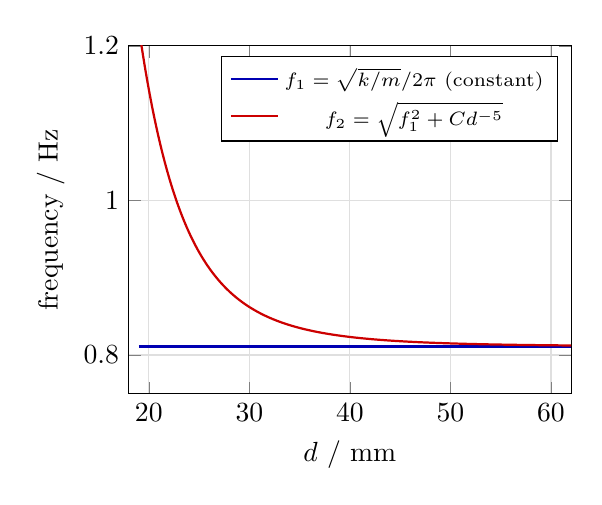
\begin{tikzpicture}
\begin{axis}[width=7.2cm,height=6cm,xlabel={$d$ / mm},ylabel={frequency / Hz},xmin=18,xmax=62,ymin=0.75,ymax=1.2,legend pos=north east,legend style={font=\scriptsize},grid=major,grid style={gray!25}]
\addplot[thick,blue!70!black,domain=19:62,samples=100]{0.811};
\addlegendentry{$f_1=\sqrt{k/m}/2\pi$ (constant)}
\addplot[thick,red!80!black,domain=19:62,samples=200]{sqrt(0.6577+2.08e6/x^5)};
\addlegendentry{$f_2=\sqrt{f_1^2+Cd^{-5}}$}
\end{axis}
\end{tikzpicture}\hfill
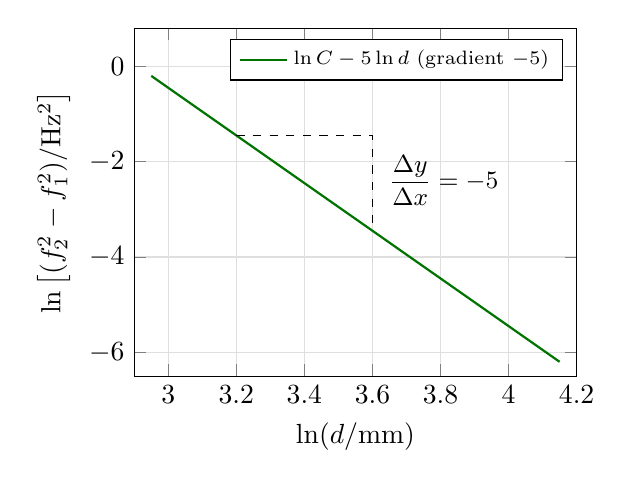
\begin{tikzpicture}
\begin{axis}[width=7.2cm,height=6cm,xlabel={$\ln(d/\mathrm{mm})$},ylabel={$\ln\big[(f_2^2-f_1^2)/\mathrm{Hz^2}\big]$},xmin=2.9,xmax=4.2,ymin=-6.5,ymax=0.8,grid=major,grid style={gray!25},legend pos=north east,legend style={font=\scriptsize}]
\addplot[thick,green!45!black,domain=2.95:4.15]{14.55-5*x};
\addlegendentry{$\ln C-5\ln d$ (gradient $-5$)}
\draw[dashed] (axis cs:3.2,-1.45)--(axis cs:3.6,-1.45)--(axis cs:3.6,-3.45);
\node[anchor=west] at (axis cs:3.62,-2.4){\small $\dfrac{\Delta y}{\Delta x}=-5$};
\end{axis}
\end{tikzpicture}\\[2pt]
{\small\textbf{Figure 10.} What the model predicts (drawn with $f_1=0.811\un{Hz}$ and the $C$ fitted to your data). Left: $f_1$ is flat, $f_2$ falls towards it as $d^{-5/2}$-ish and merges with it beyond $\sim45\un{mm}$. Right: the coupling term on log--log axes is a straight line of gradient exactly $-5$.}
\end{center}

\textbf{Why subtract the squares, rather than just look at $f_2$?} Three reasons. (i) $k$ cancels: you do not need to know the spring constant, Young's modulus, or the strip dimensions to test the force law. (ii) $f_1$ is measured in the \emph{same} record as $f_2$, so any slow drift of the springs (temperature, clamp creep) affects both and largely cancels. (iii) The result is \emph{linear} in $\gamma$, so the exponent of $d$ appears directly as the gradient of the ln--ln plot. The gradient tests the \emph{form} of the force law ($r^{-4}$ $\Rightarrow$ $-5$); the intercept $\ln C=\ln(3\muz\mum^2/\pi^3m)$ tests its \emph{magnitude} and needs $\mum$ and $m$.

\textbf{Units check.} $[\muz\mum^2]=\mathrm{T\,m\,A^{-1}\cdot A^2m^4}=\mathrm{T\,A\,m^5}$, and $1\un{T}=1\un{kg\,A^{-1}s^{-2}}$, so $[\muz\mum^2]=\mathrm{kg\,m^5s^{-2}}$. Dividing by $m$ (kg) and $d^5$ ($\mathrm{m^5}$) leaves $\mathrm{s^{-2}}$: the units of $f^2$. $C$ itself is in $\mathrm{m^5s^{-2}}$.

\begin{selfcheck}
Put numbers in. At $d=21\un{mm}$: $f_2^2-f_1^2=1.063^2-0.823^2=0.4526\un{Hz^2}$, so $\gamma/m=2\pi^2\times0.4526=8.9\un{s^{-2}}$, while $k/m=(2\pi\times0.823)^2=26.7\un{s^{-2}}$. If the dipole law held exactly, going from $21$ to $40\un{mm}$ should divide the coupling term by $(40/21)^5=25$, to $0.018\un{Hz^2}$; the measured value is $0.0145\un{Hz^2}$.
\end{selfcheck}

\begin{ownwords}
Show the subtraction, emphasise that $k$ drops out, write $f_2^2-f_1^2=Cd^{-5}$ with $C$ explicit, take logs, and say what the gradient and the intercept each test.
\end{ownwords}

\bigskip
\section{Step 8: what you actually see --- beats}

\begin{idea}
After release the motion is a \emph{mixture} of the two modes. The frequencies in the mixture ($f_1$, $f_2$) are fixed by the system; the \emph{amounts} of each mode are fixed by how you start it. An FFT peak height is simply the amount of that mode in the record, and the sum of two cosines of nearby frequency is a beat.
\end{idea}

\subsection*{8a. The general motion has two ``amounts'', $\eta_0$ and $\xi_0$}

Step 6 showed that $\eta=x_1+x_2$ and $\xi=x_1-x_2$ each obey their own SHM equation, so the most general motion is
\[
\eta(t)=\eta_0\cos(\omega_1t+\phi_1),\qquad \xi(t)=\xi_0\cos(\omega_2t+\phi_2),
\]
with four constants fixed by the four initial conditions (two positions, two velocities). Both springs start from rest, $\dot\eta(0)=\dot\xi(0)=0$, which forces $\phi_1=\phi_2=0$. The two \emph{mode amplitudes} are then just the initial values of the normal coordinates:
\begin{equation}
\eta_0=x_1(0)+x_2(0),\qquad \xi_0=x_1(0)-x_2(0).
\label{eq:amps}
\end{equation}
Transforming back with $x_1=(\eta+\xi)/2$ and $x_2=(\eta-\xi)/2$:
\begin{equation}
\boxed{\;x_1(t)=\frac{\eta_0}{2}\cos\omega_1t+\frac{\xi_0}{2}\cos\omega_2t,\qquad
x_2(t)=\frac{\eta_0}{2}\cos\omega_1t-\frac{\xi_0}{2}\cos\omega_2t\;}
\label{eq:solution}
\end{equation}
Each spring's displacement is \emph{two cosines}, one at each mode frequency, with amplitudes $\eta_0/2$ and $\xi_0/2$. Different ways of starting give different amounts:

\begin{center}\footnotesize
\begin{tabular}{@{}p{3.6cm}ccp{5.6cm}@{}}
\toprule
how you start it & $x_1(0),\ x_2(0)$ & $\eta_0,\ \xi_0$ & what you see\\
\midrule
both pushed the same way & $A,\ A$ & $2A,\ 0$ & pure in-phase mode: one frequency $f_1$, no beats\\
pushed opposite ways & $A,\ -A$ & $0,\ 2A$ & pure anti-phase mode: one frequency $f_2$, no beats\\
one displaced, other exactly at rest & $A,\ 0$ & $A,\ A$ & both modes equally: beats that go down to zero\\
one \emph{held}, other has drifted & $A,\ x_{20}$ & $A+x_{20},\ A-x_{20}$ & both modes unequally: beats that do not reach zero\\
\bottomrule
\end{tabular}
\end{center}

\begin{center}
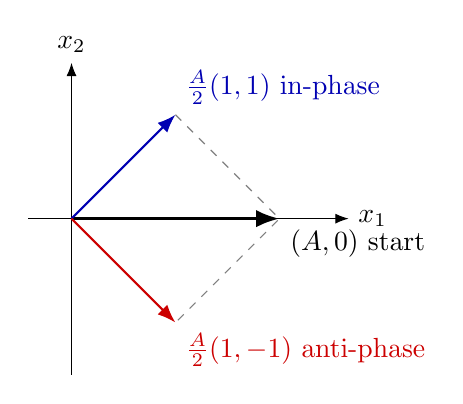
\begin{tikzpicture}[scale=1.1]
\draw[-{Latex}] (-0.5,0)--(3.2,0) node[right]{$x_1$};
\draw[-{Latex}] (0,-1.8)--(0,1.8) node[above]{$x_2$};
\draw[-{Latex},very thick,black] (0,0)--(2.4,0) node[below right]{$(A,0)$ start};
\draw[-{Latex},thick,blue!70!black] (0,0)--(1.2,1.2) node[above right]{$\tfrac A2(1,1)$ in-phase};
\draw[-{Latex},thick,red!80!black] (0,0)--(1.2,-1.2) node[below right]{$\tfrac A2(1,-1)$ anti-phase};
\draw[dashed,gray] (1.2,1.2)--(2.4,0)--(1.2,-1.2);
\end{tikzpicture}\\[2pt]
{\small\textbf{Figure 11.} The third row of the table as a picture: the starting configuration $(x_1,x_2)=(A,0)$ is the sum of equal amounts of the in-phase pattern $(1,1)$ and the anti-phase pattern $(1,-1)$. Each pattern then oscillates at its own frequency. For the fourth row the black arrow tilts up to $(A,x_{20})$ and the blue component becomes longer than the red one.}
\end{center}

\subsection*{8b. What the height of an FFT peak means}

A Fourier transform takes a record and works out which cosines it is made of; for each frequency it reports the \emph{amplitude} of the cosine at that frequency. Equation~\eqref{eq:solution} says that $x_1(t)$ is made of exactly two cosines, so its spectrum has exactly two peaks, and (for a record long enough to separate them, $T\gg1/(f_2-f_1)$) their heights are proportional to the two amplitudes:
\begin{equation}
\frac{\text{height of the $f_2$ peak}}{\text{height of the $f_1$ peak}}=\frac{\xi_0/2}{\eta_0/2}=\frac{\xi_0}{\eta_0}.
\label{eq:ratio}
\end{equation}
That is the \emph{entire} content of the ``equal heights'' remark: the peaks are equal if and only if $\eta_0=\xi_0$, i.e.\ if and only if $x_2(0)=0$. It is a statement about the starting condition, not about the modes. Two consequences matter for the essay:
\begin{itemize}[nosep]
\item The \emph{positions} of the peaks, $f_1$ and $f_2$, do not depend on the starting condition at all. That is why one FFT of one spring gives both mode frequencies whatever the exact release---the method never needed equal heights, only that both modes are present.
\item The \emph{heights} tell you about the starting condition and (8f) about whether the two springs are identical.
\end{itemize}

\subsection*{8c. Why your peaks are \emph{not} equal --- and why that is correct}

You observed that the $f_2$ peak is only about $0.6$ of the $f_1$ peak and that the beats do not go down to zero. Both follow from how a spring is really released. You do not flick spring~1 instantaneously from $0$ to $A$: you \emph{hold} it at $A$ for a moment and then let go. While it is held the separation of the magnets is different, so the repulsion on spring~2 is different, and spring~2 quietly moves to a new rest position \emph{before} you release. Setting $\ddot x_2=0$ in the equation of motion of spring~2 (Step~5) with $x_1=A$:
\[
0=-kx_2-\gamma(x_2-A)\qquad\Longrightarrow\qquad x_{20}=\frac{\gamma}{k+\gamma}\,A,
\]
in the same direction as $A$ (spring~2 is pushed away if you push spring~1 towards it, and follows if you pull spring~1 away). By \eqref{eq:amps}, $\eta_0=A+x_{20}$ and $\xi_0=A-x_{20}$, so by \eqref{eq:ratio}
\begin{equation}
\boxed{\;\frac{\text{height at }f_2}{\text{height at }f_1}=\frac{A-x_{20}}{A+x_{20}}=\frac{k}{k+2\gamma}=\frac{\omega_1^2}{\omega_2^2}=\Big(\frac{f_1}{f_2}\Big)^2\;}
\label{eq:hold}
\end{equation}
With your $f_1=0.802$ and $f_2=0.996\un{Hz}$ this is $0.65$; you measured about $0.58$. The remaining difference is about the size of the non-linear correction: with the full $r^{-4}$ force instead of its tangent, a $10\un{mm}$ hold gives $0.49$ if spring~1 was pushed \emph{towards} spring~2 and $0.71$ if it was pulled \emph{away} ($A=10\un{mm}$ is not small compared with $d=23\un{mm}$). So a ratio around $0.6$ is exactly what a real hold-and-release should give. It is not an error to be fixed, it does not move $f_1$ or $f_2$, and in the essay you can quote \eqref{eq:hold} as a small extra check of the model. The envelope minima follow too: the amplitude swings between $(\eta_0+\xi_0)/2=A$ and $(\eta_0-\xi_0)/2=x_{20}$, so minimum/maximum $=x_{20}/A=\gamma/(k+\gamma)\approx0.2$ instead of $0$.

\begin{center}
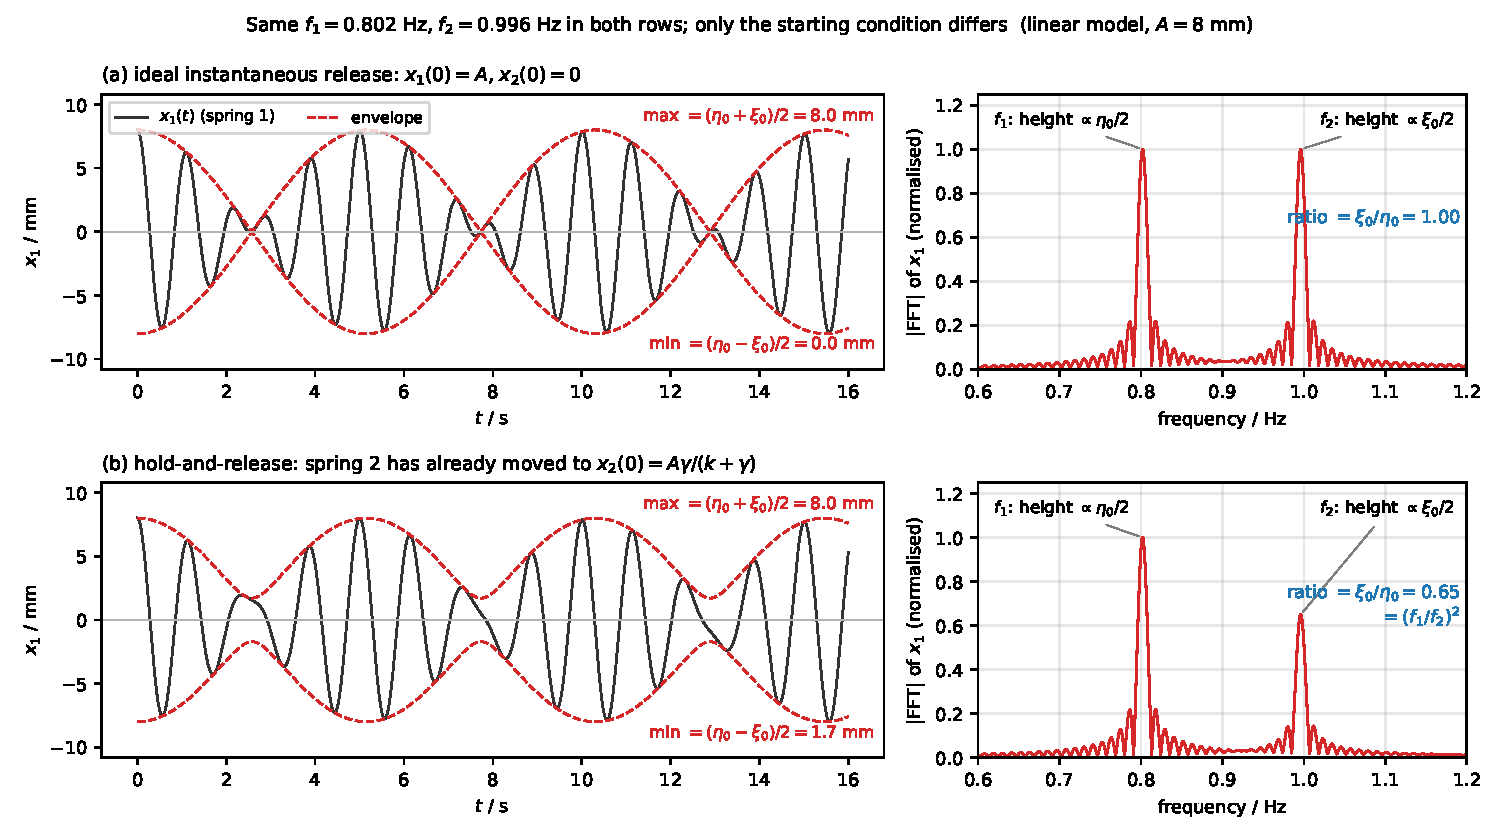
\includegraphics[width=\textwidth]{fig_release.pdf}\\[2pt]
{\small\textbf{Figure 12.} The same system ($f_1=0.802$, $f_2=0.996\un{Hz}$) started in two ways (linear model). Top: idealised instantaneous release, $x_2(0)=0$: equal mode amplitudes, equal FFT peaks, beats that touch zero. Bottom: hold-and-release, $x_2(0)=A\gamma/(k+\gamma)=1.7\un{mm}$: peak ratio $(f_1/f_2)^2=0.65$ and envelope minima of $1.7\un{mm}$ instead of zero. The peak \emph{positions} are identical in both rows.}
\end{center}

\subsection*{8d. Two cosines make a beat: the rotating-arrow picture}

Write each cosine as the horizontal projection of a rotating arrow (a phasor). Arrow~1 has length $\eta_0/2$ and turns at $f_1$ revolutions per second; arrow~2 has length $\xi_0/2$ and turns at $f_2$ revolutions per second; $x_1$ is the horizontal projection of their vector sum (Figure~13). Because arrow~2 turns slightly faster, the angle between them grows steadily, by $f_2-f_1$ revolutions every second. When they point the same way the sum is long, $(\eta_0+\xi_0)/2$; half a relative turn later they oppose each other and the sum is short, $|\eta_0-\xi_0|/2$; after one full relative turn they are aligned again. So the amplitude of the fast oscillation swells and shrinks with period
\begin{equation}
\boxed{\;T_{\rm beat}=\frac{1}{f_2-f_1},\qquad f_{\rm beat}=f_2-f_1\;}
\end{equation}
\emph{whatever the two lengths are}; the lengths only decide how deep the minima go (zero for equal lengths, $x_{20}$ for the hold-and-release). Meanwhile the sum-arrow itself turns at about the average rate, which is the fast oscillation at $f_{\rm avg}=(f_1+f_2)/2$ (exactly that for equal lengths).

\begin{center}
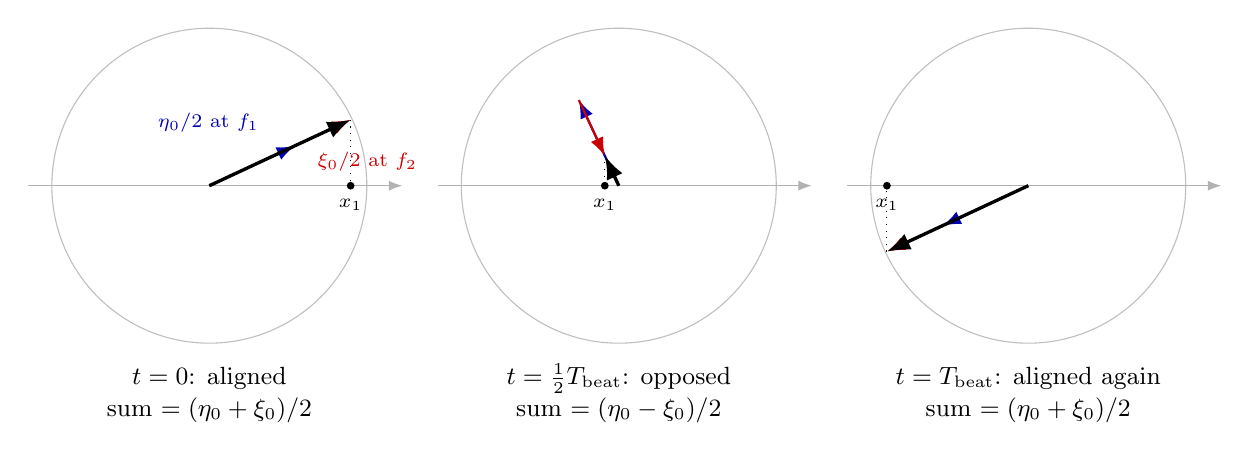
\begin{tikzpicture}[scale=1.0]
% blue arrow: length 1.2 at angle ta; red arrow: length 0.78 at angle tb (relative angle 0, 180, 360)
\foreach \dx/\ta/\tb/\capA/\capB in {0/25/25/{$t=0$: aligned}/{sum $=(\eta_0+\xi_0)/2$},
                                     5.2/115/295/{$t=\tfrac12T_{\rm beat}$: opposed}/{sum $=(\eta_0-\xi_0)/2$},
                                     10.4/205/205/{$t=T_{\rm beat}$: aligned again}/{sum $=(\eta_0+\xi_0)/2$}}{
 \begin{scope}[shift={(\dx,0)}]
  \draw[gray!50] (0,0) circle (2.0);
  \draw[gray!60,-{Latex}] (-2.3,0)--(2.45,0);
  \draw[-{Latex},thick,blue!70!black] (0,0)--(\ta:1.2) coordinate (p);
  \draw[-{Latex},thick,red!80!black] (p)--++(\tb:0.78) coordinate (q);
  \draw[-{Latex},very thick,black] (0,0)--(q);
  \draw[dotted] (q)--(q|-0,0);
  \fill (q|-0,0) circle (1.4pt);
  \node[below,font=\scriptsize] at ($(q|-0,0)+(0,-0.05)$) {$x_1$};
  \node[align=center,font=\small] at (0,-2.45) {\capA};
  \node[align=center,font=\small] at (0,-2.85) {\capB};
 \end{scope}
}
\node[blue!70!black,font=\scriptsize,anchor=south east] at (0.75,0.55) {$\eta_0/2$ at $f_1$};
\node[red!80!black,font=\scriptsize,anchor=north west] at (1.25,0.55) {$\xi_0/2$ at $f_2$};
\end{tikzpicture}\\[2pt]
{\small\textbf{Figure 13.} Beats as rotating arrows. Blue: length $\eta_0/2$, turning at $f_1$ rev/s. Red (drawn head-to-tail): length $\xi_0/2$, turning at $f_2$ rev/s. Black: their sum; $x_1$ is its horizontal projection. The relative angle grows by one full turn every $1/(f_2-f_1)$ seconds, so the length of the black arrow---the amplitude of the fast oscillation---repeats with exactly that period. Lengths drawn for $\xi_0/\eta_0=0.65$ (the hold-and-release); the sum never shrinks to zero.}
\end{center}

\subsection*{8e. The same thing with a trig identity (equal amplitudes)}

For $\eta_0=\xi_0=A$ the product-to-sum identity $\cos\alpha+\cos\beta=2\cos\frac{\alpha-\beta}{2}\cos\frac{\alpha+\beta}{2}$, with $\alpha=2\pi f_1t$ and $\beta=2\pi f_2t$, turns $x_1$ into
\begin{equation}
\boxed{\;x_1(t)=A\cos\!\big(\pi(f_2-f_1)\,t\big)\;\cos\!\big(2\pi f_{\rm avg}\,t\big),\qquad f_{\rm avg}=\frac{f_1+f_2}{2}\;}
\label{eq:beats}
\end{equation}
Read this as \emph{[slowly varying amplitude]} $\times$ \emph{[fast oscillation]}: the second factor is the fast oscillation at the average frequency, the first is the envelope (Figure~14).

\begin{center}
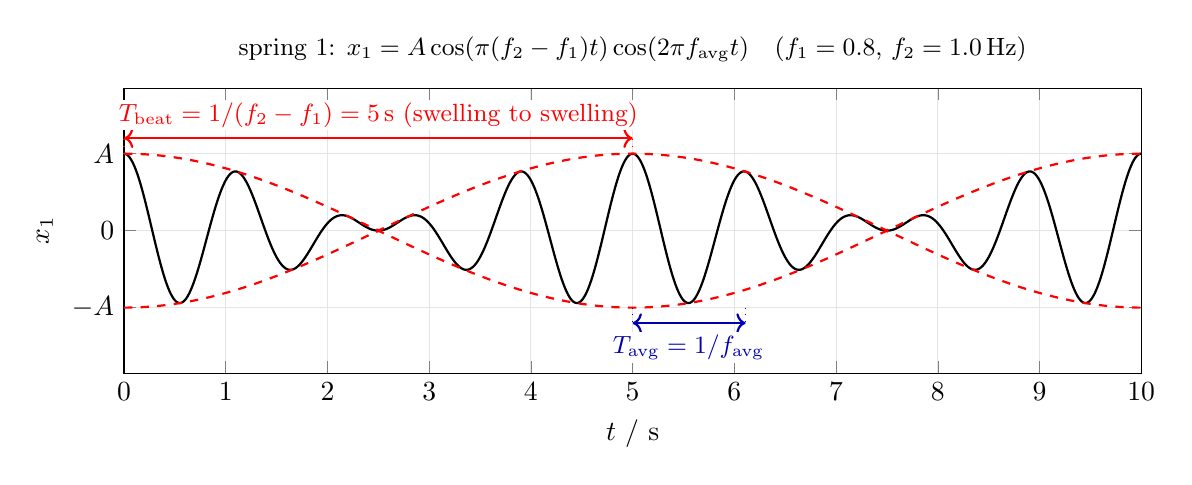
\begin{tikzpicture}
\begin{axis}[width=14.5cm,height=5.2cm,xlabel={$t$ / s},ylabel={$x_1$},xmin=0,xmax=10,ymin=-1.85,ymax=1.85,ytick={-1,0,1},yticklabels={$-A$,$0$,$A$},grid=major,grid style={gray!20},clip=false,title={\small spring 1: $x_1=A\cos(\pi(f_2-f_1)t)\cos(2\pi f_{\rm avg}t)$\quad ($f_1=0.8$, $f_2=1.0\un{Hz}$)}]
\addplot[thick,black,domain=0:10,samples=700]{cos(deg(0.2*pi*x))*cos(deg(1.8*pi*x))};
\addplot[thick,red,dashed,domain=0:10,samples=300]{abs(cos(deg(0.2*pi*x)))};
\addplot[thick,red,dashed,domain=0:10,samples=300]{-abs(cos(deg(0.2*pi*x)))};
\draw[dotted,red] (axis cs:0,1)--(axis cs:0,1.25); \draw[dotted,red] (axis cs:5,1)--(axis cs:5,1.25);
\draw[<->,thick,red] (axis cs:0,1.2)--(axis cs:5,1.2);
\node[red,fill=white,inner sep=1pt] at (axis cs:2.5,1.5){\small $T_{\rm beat}=1/(f_2-f_1)=5\un{s}$ (swelling to swelling)};
\draw[dotted,blue!70!black] (axis cs:5,-1)--(axis cs:5,-1.25); \draw[dotted,blue!70!black] (axis cs:6.111,-1)--(axis cs:6.111,-1.25);
\draw[<->,thick,blue!70!black] (axis cs:5,-1.2)--(axis cs:6.111,-1.2);
\node[blue!70!black,fill=white,inner sep=1pt] at (axis cs:5.55,-1.52){\small $T_{\rm avg}=1/f_{\rm avg}$};
\end{axis}
\end{tikzpicture}\\
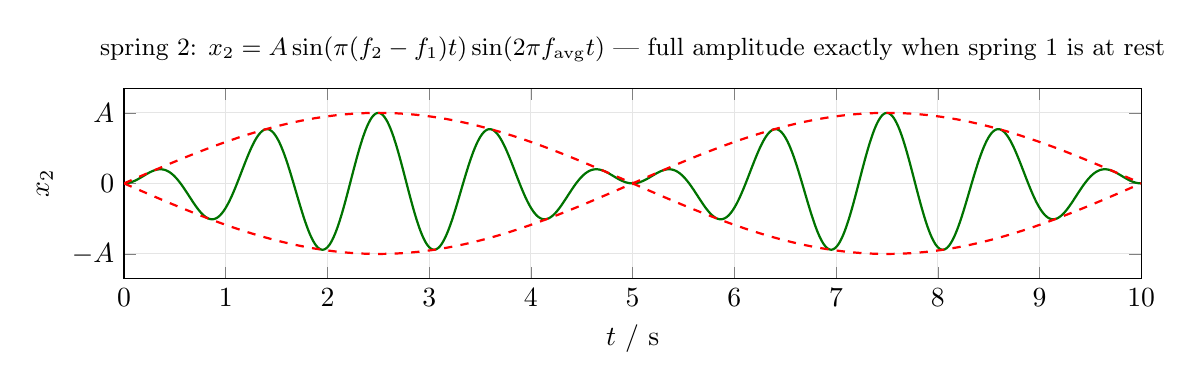
\begin{tikzpicture}
\begin{axis}[width=14.5cm,height=4.0cm,xlabel={$t$ / s},ylabel={$x_2$},xmin=0,xmax=10,ymin=-1.35,ymax=1.35,ytick={-1,0,1},yticklabels={$-A$,$0$,$A$},grid=major,grid style={gray!20},title={\small spring 2: $x_2=A\sin(\pi(f_2-f_1)t)\sin(2\pi f_{\rm avg}t)$ --- full amplitude exactly when spring 1 is at rest}]
\addplot[thick,green!45!black,domain=0:10,samples=700]{sin(deg(0.2*pi*x))*sin(deg(1.8*pi*x))};
\addplot[thick,red,dashed,domain=0:10,samples=300]{abs(sin(deg(0.2*pi*x)))};
\addplot[thick,red,dashed,domain=0:10,samples=300]{-abs(sin(deg(0.2*pi*x)))};
\end{axis}
\end{tikzpicture}\\[2pt]
{\small\textbf{Figure 14.} Beats for equal mode amplitudes. Top: the released spring (black) and its envelope (red dashed). The envelope cosine has frequency $(f_2-f_1)/2$, but its \emph{modulus} peaks twice per cycle, so the swellings recur every $T_{\rm beat}=1/(f_2-f_1)$---the same conclusion as the arrow picture. Bottom: spring~2 is a quarter of a beat behind; it has all the energy when spring~1 has none.}
\end{center}

\begin{pitfall}
``Is the beat frequency $f_2-f_1$ or $(f_2-f_1)/2$?'' Both numbers appear and they mean different things. The \emph{envelope function} $\cos(\pi(f_2-f_1)t)$ has frequency $(f_2-f_1)/2$. But an amplitude cannot be negative: what you see is $|\cos|$, which has maxima twice per cycle. The time between two swellings---what you measure on the Tracker plot---is $1/(f_2-f_1)$ (the arrow picture gives this directly, with no sign ambiguity). So the observable beat frequency is
\[
f_{\rm beat}=f_2-f_1=\frac1{T_{\rm beat}},\qquad
f_2^2-f_1^2=(f_2-f_1)(f_2+f_1)=2\,f_{\rm beat}\,f_{\rm avg}.
\]
Use this convention consistently; it is the one used in the essay (Figure 3, Section 5.4, Graph 4).
\end{pitfall}

\subsection*{8f. Spring 2, and a test for identical springs}

Spring~2 contains the same two cosines with the sign of the anti-phase term reversed (equation~\eqref{eq:solution}). Three consequences:
\begin{enumerate}[nosep,leftmargin=1.6em]
\item Its FFT has peaks at the \emph{same} $f_1$, $f_2$, with the \emph{same} height ratio $\xi_0/\eta_0$---for identical springs this holds for any starting condition, because each mode has the same amplitude in both springs (mode shapes $(1,1)$ and $(1,-1)$).
\item For equal amplitudes, $x_2=A\sin(\pi(f_2-f_1)t)\sin(2\pi f_{\rm avg}t)$: its envelope is a quarter of a beat behind that of spring~1, so spring~2 is at full swing when spring~1 is quiet (Figure~14, bottom). This is the energy transfer of the introduction.
\item If the springs are \emph{not} identical, the mode shapes tilt to $(a_1,b_1)$ and $(-b_1,a_1)$ with $a_1\neq b_1$, and the height ratios of the two springs differ: $r_2/r_1=(a_1/b_1)^2$, with $a_1/b_1-b_1/a_1=2\Delta/\kappa$ in the notation of essay Section~10.4. Your spectra show $r_2$ slightly larger than $r_1$ (about $10\,\%$), which corresponds to a stiffness mismatch of order $1\,\%$ with spring~2 the stiffer one---the cleanest test of assumption~(c) you have, and much smaller than the $7\,\%$ the detuned fit suggested.
\end{enumerate}

\subsection*{8g. Predictions for $f_{\rm avg}$ and $f_{\rm beat}$}
Combining $f_2=\sqrt{f_1^2+Cd^{-5}}$ with the definitions:
\begin{equation}
f_{\rm beat}=\sqrt{f_1^2+Cd^{-5}}-f_1=\frac{Cd^{-5}}{2f_{\rm avg}},\qquad
f_{\rm avg}=\frac{f_1+\sqrt{f_1^2+Cd^{-5}}}{2}.
\end{equation}
Because $f_{\rm avg}$ only varies between $f_1$ and about $1.15f_1$, the beat frequency falls almost exactly as $d^{-5}$ (for weak coupling $f_{\rm beat}\approx Cd^{-5}/2f_1$), while the average frequency is nearly constant and rises only at small $d$. With your numbers: $T_{\rm beat}\approx4\un{s}$ at $21\un{mm}$, $\approx110\un{s}$ at $40\un{mm}$, and the dipole law predicts about ten \emph{minutes} at $60\un{mm}$---which is why no beats (and no second peak) were seen there in a $30\un{s}$ record.

\begin{ownwords}
(1) After release the motion is a superposition of the two modes; starting from rest, the mode amplitudes are $\eta_0=x_1(0)+x_2(0)$ and $\xi_0=x_1(0)-x_2(0)$. (2) Each spring's displacement is therefore two cosines at $f_1$ and $f_2$ with amplitudes $\eta_0/2$ and $\xi_0/2$, so an FFT of one spring shows both frequencies; the peak heights are in the ratio $\xi_0/\eta_0$ and say nothing about $f_1$, $f_2$ themselves. (3) For the hold-and-release actually used, $x_2(0)=A\gamma/(k+\gamma)$, giving a height ratio $(f_1/f_2)^2\approx0.65$ and beats whose minima are not zero---consistent with what was observed. (4) Two cosines of nearby frequency beat: fast oscillation at $f_{\rm avg}=(f_1+f_2)/2$, amplitude swelling every $T_{\rm beat}=1/(f_2-f_1)$, so $f_{\rm beat}=f_2-f_1$ and $f_2^2-f_1^2=2f_{\rm beat}f_{\rm avg}$. (5) Spring~2 carries the same two frequencies with the anti-phase term reversed, so it swings most when spring~1 is quiet; identical springs give the same height ratio in both spectra, non-identical springs do not.
\end{ownwords}

\bigskip

\section{The assumptions, and why each one matters}

\begin{center}\small
\begin{tabular}{@{}p{0.5cm}p{4.6cm}p{5.3cm}p{5.0cm}@{}}
\toprule
 & Assumption & Where it entered & What happens if it fails\\
\midrule
(a) & magnets are point dipoles ($d\gg D$) & Step 2, $F\propto r^{-4}$ & force falls less steeply at small $d$; gradient shallower than $-5$ (essay 10.3)\\
(b) & displacements small ($A\ll d$) & Step 4, tangent instead of curve & frequency depends on amplitude; $f_2$ pushed up at small $d$ (essay 10.2)\\
(c) & the two springs are identical & Step 6, adding/subtracting works only if $k,m$ equal & $f_1$ no longer constant; peak-height ratio differs between the two springs; coupling term saturates at large $d$ (essay 10.4)\\
(d) & one spring = one lumped mass & Step 1 & small error in $m$; higher bending modes appear as extra (much higher) peaks\\
(e) & no damping & Steps 6, 8 & amplitude decays; FFT peaks broaden; frequencies shift negligibly\\
(f) & magnets stay coaxial & Step 2 (on-axis field) & tip of a bent cantilever tilts; $\lesssim1\%$ effect, independent of $d$\\
(g) & the FFT returns the true frequencies & not in the theory, but in the test of it & two close peaks pull together/merge for short records (essay 6, 10.1)\\
\bottomrule
\end{tabular}
\end{center}

\section{Symbols}

\begin{center}\footnotesize
\begin{tabular}{@{}p{3.1cm}p{4.1cm}p{3.6cm}p{4.9cm}@{}}
\toprule
Symbol & Meaning & Symbol & Meaning\\
\midrule
$L,b,h$ & length, width, thickness of a spring & $d$ & equilibrium centre-to-centre separation\\
$E$, $I=bh^3/12$ & Young's modulus, second moment of area & $\delta$ & static outward bend of each spring, $k\delta=F(d)$\\
$k=3EI/L^3$ & tip stiffness of a spring & $x_1,x_2$ & displacements from equilibrium (same sign convention)\\
$M,\ \mu$ & magnet mass, strip mass per length & $r=d+x_2-x_1$ & instantaneous separation\\
$m=M+\frac{33}{140}\mu L$ & effective oscillating mass & $\gamma=-F'(d)$ & magnetic stiffness $=6\muz\mum^2/\pi d^5$\\
$\mum$ & dipole moment of a magnet & $\eta=x_1+x_2$, $\xi=x_1-x_2$ & normal coordinates\\
$\muz$ & permeability of free space & $\omega_1^2=k/m$, $\omega_2^2=(k+2\gamma)/m$ & mode angular frequencies\\
$F(r)=3\muz\mum^2/2\pi r^4$ & repulsive force & $C=3\muz\mum^2/\pi^3m$ & constant in $f_2^2-f_1^2=Cd^{-5}$\\
$f_{\rm avg}=(f_1+f_2)/2$ & average frequency & $f_{\rm beat}=f_2-f_1=1/T_{\rm beat}$ & beat frequency\\
\bottomrule
\end{tabular}
\end{center}

\section{The argument in ten sentences (skeleton to expand in your own words)}

\begin{enumerate}[nosep,leftmargin=1.6em]
\item A clamped leaf spring pushed at its tip obeys Hooke's law with $k=3EI/L^3$, and the tip mass that oscillates is the magnet plus $33/140$ of the strip's mass.
\item Each spring alone is therefore a simple harmonic oscillator with $\omega_0^2=k/m$.
\item Treating each magnet as a point dipole, the on-axis field falls as $r^{-3}$ and the repulsion between the two like-facing magnets is $F=3\muz\mum^2/(2\pi r^4)$.
\item At equilibrium the repulsion bends each spring outwards by $\delta$ with $k\delta=F(d)$; $d$ is defined and measured in this state, and displacements $x_1,x_2$ are counted from it.
\item For small displacements the change in the repulsion is proportional to the change in separation, $\Delta F=-\gamma\Delta r$, with $\gamma=-F'(d)=4F(d)/d\propto d^{-5}$: the magnetic field acts as a spring of stiffness $\gamma$ between the magnets.
\item Newton's second law for each magnet, after the equilibrium force cancels, gives $m\ddot x_1=-kx_1+\gamma(x_2-x_1)$ and $m\ddot x_2=-kx_2-\gamma(x_2-x_1)$---two masses joined by a third spring.
\item Adding and subtracting decouples them: $x_1+x_2$ oscillates at $\omega_1^2=k/m$ (in phase, magnets keep their distance, coupling irrelevant) and $x_1-x_2$ at $\omega_2^2=(k+2\gamma)/m$ (anti-phase, separation changes twice as fast as each magnet moves, hence $2\gamma$).
\item Subtracting the squared frequencies eliminates $k$: $f_2^2-f_1^2=\gamma/(2\pi^2m)=Cd^{-5}$, so $\ln(f_2^2-f_1^2)$ against $\ln d$ should be a straight line of gradient $-5$; the intercept gives $C=3\muz\mum^2/\pi^3m$.
\item Releasing one spring from rest excites both modes (with amplitudes $\eta_0=x_1(0)+x_2(0)$ and $\xi_0=x_1(0)-x_2(0)$, equal only for an instantaneous release), so each magnet's motion is $\frac{\eta_0}{2}\cos\omega_1t\pm\frac{\xi_0}{2}\cos\omega_2t$: a fast oscillation at $f_{\rm avg}=(f_1+f_2)/2$ whose amplitude beats at $f_{\rm beat}=f_2-f_1$, with energy passing back and forth between the springs; an FFT of either spring shows two peaks at $f_1$ and $f_2$ whose height ratio $\xi_0/\eta_0$ reflects only the starting condition.
\item The derivation assumed point dipoles, small amplitudes, identical springs, a lumped mass, no damping and coaxial magnets; each assumption is examined in the evaluation.
\end{enumerate}

\section*{Answers to the ``check yourself'' questions and two more}

\begin{description}[leftmargin=0pt,itemsep=3pt]
\item[Why does $k$ cancel?] Because $\omega_1^2$ and $\omega_2^2$ both contain $k/m$ and differ only by $2\gamma/m$. This is the reason for using $f_2^2-f_1^2$ rather than $f_2$ alone.
\item[Why the factor 2 in $k+2\gamma$?] In the anti-phase mode each magnet moves $a$ but the separation changes by $2a$; the magnetic spring responds to the separation, so it exerts $2\gamma a$ on each magnet.
\item[Why does $f_1$ not depend on $d$?] In the in-phase mode the separation never changes, so the magnetic force stays at its constant equilibrium value, which is already balanced by the static bend $\delta$.
\item[Why $-5$ and not $-4$?] The force is $\propto r^{-4}$, but the frequency shift depends on the \emph{stiffness}, the derivative of the force, which is $\propto r^{-5}$.
\item[Why are the two FFT peaks not equal in height?] Their heights are the amplitudes $\eta_0/2$ and $\xi_0/2$ of the two modes, fixed by the starting positions: equal only if $x_2(0)=0$. Holding spring~1 at $A$ lets spring~2 drift to $x_{20}=A\gamma/(k+\gamma)$ first, so the ratio is $(A-x_{20})/(A+x_{20})=(f_1/f_2)^2\approx0.65$, and the beats no longer reach zero. Neither effect changes $f_1$ or $f_2$.
\end{description}

\end{document}
